\section{Improving stability via average margin interpolation}

In this section we discuss how in high dimensions, the error of the
min-$\ell_1$-margin solution is not optimal even when the ground truth is
sparse. Our synthetic experiments reveal how this phenomenon is particularly
pronounced in high dimensions and provide insights into its causes.


\subsection{High-dimensional setting}
\label{sec:setting}

We consider training data $\DD=\{(x_i, y_i)\}_{i=1}^{n}$ for a binary
classification problem, with $x\in \RR^d$ and $y\in \{-1, +1\}$. We focus
primarily on high-dimensional settings, i.e.\ $d \gg n$ and assume that the
covariates are drawn from a mixture of two truncated Gaussians, each of them
corresponding to one of the two classes. We assume
that the data is noiseless, and hence, there exists a linear classifier with
vanishing Bayes error. Without loss of generality, we assume the Bayes optimal
classifier to be $\thetastar=e_1=[1, 0, ..., 0] \in \RR^d$. We also present
experiments for a $5$-sparse ground truth.

We are interested in analyzing the estimation error of a classifier $\thetahat$,
which captures how well $\thetahat$ recovers the ground truth:

\begin{align}
\err(\thetahat) = \|\thetahat - \thetastar\|_2^2 
\end{align}

Naturally, good estimation error implies good prediction performance as well.


\subsection{Min-margin interpolation}

Consider the estimator that maximizes the min-$\ell_1$-margin of the training
data:

\begin{align}
  \mm =& \arg\max_{\theta} \min_{(x_i, y_i) \in \DD} y_i\theta^\top x_i \\
  &\st
  \|\theta\|_1 \le 1 \text{ and } y_i\theta^\top x_i > 0, \forall i \in [n]
\end{align}

We note that this estimator coincides with the solution to the hard
$\ell_1$-margin SVM problem:

\begin{align}
  \mm = \arg\min_{\theta} \|\theta\|_1 \st y_i\theta^\top x_i \ge 1, \forall i \in
  [n]
\end{align}

\subsection{The problem with min-margin interpolation}

The work of \citet{konstantin} reveals a problem that min-$\ell_1$-margin
interpolation exhibits in high dimensions.  To showcase this issue, let us
compare it to min-l2-margin interpolation, which, unlike the former, lacks the
inductive bias that is expected to make it easier to recover the sparse ground
truth. Despite not having the appropriate inductive bias, \citet{konstantin}
show that the min-l2-margin solution can actually achieve better estimation
error in high dimensions. 
% In particular, as also observed by [TODO konstantin], in the presence of label
% noise, min-l1-margin interpolation achieves worse performance compared to its
% $\ell_2$ counterpart.  As Figure~\at{TODO} reveals,
This failure of is, in large part, due to an increase in the variance of the
min-$\ell_1$-margin solution, despite having a significantly lower bias.

Next we propose an alternative to maximizing the min-$\ell_1$-margin which is
specifically designed to have lower variance in high dimensions.  Surprisingly,
we see that this alternative interpolator also reduces the bias, leading to
smaller estimation error compared to the min-margin solution, even in the
noiseless case.


\begin{figure*}[t]
  \centering
  \begin{subfigure}[t]{0.24\linewidth}
    \centering
    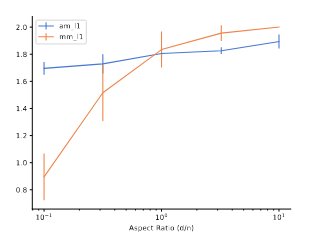
\includegraphics[width=\columnwidth]{figures/estim_err_outlier1.png}
    \label{fig:estim_err_outlier1}
    \caption{}
  \end{subfigure}
  \hfill
  \begin{subfigure}[t]{0.24\linewidth}
    \centering
    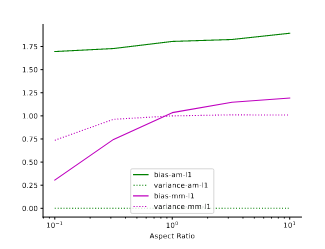
\includegraphics[width=\columnwidth]{figures/bias_variance_outlier1.png}
    \label{fig:bias_variance_outlier1}
    \caption{}
  \end{subfigure}
  \hfill
  \begin{subfigure}[t]{0.24\linewidth}
    \centering
    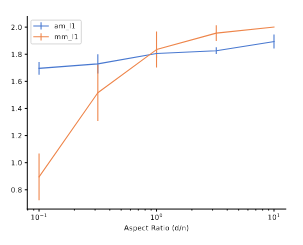
\includegraphics[width=\columnwidth]{figures/estim_err_outlier2.png}
    \label{fig:estim_err_outlier2}
    \caption{}
  \end{subfigure}
  \hfill
  \begin{subfigure}[t]{0.24\linewidth}
    \centering
    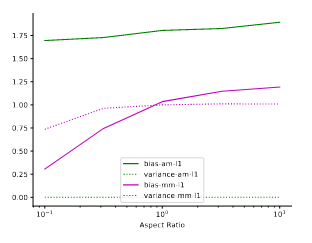
\includegraphics[width=\columnwidth]{figures/bias_variance_outlier2.png}
    \label{fig:bias_variance_outlier2}
    \caption{}
  \end{subfigure}

  \caption{In low dimensions and in the presence of outliers, the average-margin
    solution can have significantly larger estimation error compared to
    min-margin interpolation. Surprisingly, the average-margin classifier is
    more robust in high dimensions (i.e.\ aspect ratio greater than $1$). For
    all experiments we set $d=???$\at{TODO}.} \label{fig:limitations}

\end{figure*}

\subsection{Average-margin interpolation}

In order to reduce the variance of the max-$\ell_1$-margin interpolator, we
propose to study a different interpolating estimator, which maximizes the
\emph{average} $\ell_1$ margin instead of the \emph{minimum} $\ell_1$ margin:

\begin{align}
  \am =& \arg\max_{\theta} \frac{1}{n} \sum_{(x_i, y_i) \in \DD} y_i\theta^\top x_i \\
  &\st
  \|\theta\|_1 \le 1 \text{ and } y_i\theta^\top x_i > 0, \forall i \in [n]
\end{align}

Unlike the min-margin interpolator, the average-margin solution is determined
by \emph{all} the points in the training set. Intuitively, this dependence of
the classifier on all samples is expected to reduce the variance, since it is
less likely that a single point will exert a large influence over the solution
of the optimization problem. This lower variance, combined with the low bias
(which is a consequence of using the $\ell_1$ norm), can decrease the estimation
error compared to min-margin interpolation.


\subsection{Experiments}

We compare average-$\ell_1$-margin and min-$\ell_1$-margin maximization on the
classification problem introduced in Section \at{TODO}. We consider $d=???$ ...
\at{TODO Gizem: describe l1-mm vs l2-mm experiment setting: fixed d, vary n,
how we compute the solutions}. We consider 1-sparse and 5-sparse ground truths.

The main experimental results are illustrated in Figure~\at{TODO}. First, we
notice that the estimation error is significantly reduced by solving the
average-margin optimization problem. Second, the simulations confirm that indeed
the variance of the average-margin solution is much smaller than for the
min-margin interpolator. For a 5-sparse ground truth, the trends remain similar,
with the only mention that the error is slightly larger at the
same $d/n$ ratio. This is expected as the same information (i.e.\ same number of
training samples) is now used to predict more parameters (i.e.\ the $5$
coefficients of the support of $\thetastar$).

In addition, perhaps surprisingly, we notice that avg-margin interpolation also
reduces the bias, which further decreases the error. We leave as future work a
thorough investigation of the mechanism through which average-margin
interpolation leads to lower bias.
% A similar phenomenon has been observed by [TODO our RO paper] where the
% authors note that the 1-sparse ground truth has high average margin, but low
% min margin. 
% Therefore, average-margin maximization is more suitable for recovering
% $\thetastar$.

\subsection{Emergence of average-margin classifiers in practice}

So far we have focused solely on linear models, and hence, a natural question is
whether the insights that we have presented in this section carry over to more
complex classifiers, like deep neural networks.

% Finally, we note that we expect that the insights that we gain using linear
% models carries over to more complex classifiers, like overparameterized deep
% neural networks trained with a suitable loss.
For simplicity, we only study the solution of a convex optimization problem that
we obtain using standard solvers for linear and quadratic programs. However,
prior work allows us to connect the average-margin classifier to certain
predictors that can be achieved in practice.  In particular, \citet{wang21} show
that minimizing a polynomially-tailed loss leads to an estimator akin to the
average-margin solution from Equation~\at{blabla}. Furthermore, \citet{ro}
suggest that conventional regularization techniques like a ridge penalty or
early stopping favor solutions with high average margin (as opposed to the
solution with large min-margin that is found at convergence). In fact, given
that an estimator $\thetahat$ has small norm, writing the Taylor expansion of
the logistic loss leads to precisely the average margin of Equation~\at{bla}.
We leave as future work a thorough analysis of the benefits of maximizing the
average-margin in the context of deep neural networks in the low-sample regime.

